\documentclass{article}
\usepackage{hyperref} % 可选:添加超链接支持
\usepackage{graphicx}

\usepackage{xr}
\externaldocument{sum1}

\usepackage{indentfirst}
\setlength{\parindent}{2em}  % 用于首行缩进

\usepackage{amsmath}
\usepackage{enumerate}
\usepackage{mathtools}
\usepackage{amsthm} % 使用定理环境
\usepackage{amssymb}

\usepackage{bm}
\usepackage{pdfpages}
\usepackage{tabu}
\usepackage{multirow}
\usepackage{multicol}
\usepackage{float}
\usepackage{makecell}
\usepackage{booktabs}
\usepackage{url}

\usepackage[style=ieee]{biblatex} % 或 \usepackage{natbib}
\addbibresource{ec.bib} % 指定参考文献数据库


% 自定义 e-companion 的编号格式(例如 EC Section 1)
\renewcommand{\thesection}{EC.\arabic{section}} % 节编号格式:EC.1, EC.2
\renewcommand{\thefigure}{EC.\arabic{figure}}   % 图编号格式:EC.1, EC.2
\renewcommand{\thetable}{EC.\arabic{table}}    % 表编号格式:EC.1, EC.2

\newenvironment{pf}[1]{\noindent\textbf{#1}\par\medskip}{\hfill $\blacksquare$\par\medskip}
\newtheorem{corollary}{\hspace{2em}Corollary}
\newtheorem{prop}{\hspace{2em}Proposition}

% 自定义定理样式:编号格式为 EC.X,并保留缩进
\newtheoremstyle{ecompanion} % 样式名
  {2em}                     % 上方间距
  {2em}                     % 下方间距
  {\normalfont}             % 正文字体
  {}                        % 缩进(由\hspace控制)
  {\bfseries}               % 标题字体
  {.}                       % 标题后标点
  {5pt plus 1pt minus 1pt}  % 标题后间距
  {\thmname{#1}\thmnumber{ EC.#2}\thmnote{ (#3)}} % 编号格式

% 应用样式并定义 lemma 环境
\theoremstyle{ecompanion}
\newtheorem{lem}{Lemma} % 自动添加 EC. 前缀

\usepackage[linesnumbered,tworuled]{algorithm2e}
\SetKwComment{Comment}{/* }{ */}
% ===== 关键修改:重定义算法编号格式 =====
\makeatletter
\renewcommand{\fnum@algocf}{Algorithm EC.\thealgocf} % 添加 EC. 前缀
\makeatother
\RestyleAlgo{ruled}

\begin{document}

% 标题注明这是 e-companion
\title{Electronic Companion to \\ \textit{Seating Management under Social Distancing}}
\author{}
\date{}
\maketitle

% 补充内容

% !TEX root = sum1.tex

\section{Policies for Dynamic Situations}\label{policies}

\subsubsection*{Bid-price Control}
Bid-price control is a classical approach discussed extensively in the literature on network revenue management. It involves setting bid prices for different group types, which determine the eligibility of groups to take the seats. Bid-prices refer to the opportunity costs of taking one seat. As usual, we estimate the bid price of a seat by the shadow price of the capacity constraint corresponding to some row. In this section, we will demonstrate the implementation of the bid-price control policy. 

The dual of LP relaxation of problem \eqref{deter_upper} is:

\begin{equation}\label{bid-price_dual}
  \begin{aligned}
  \min \quad & \sum_{i=1}^{M} d_i z_i + \sum_{j= 1}^{N} L_j \beta_{j} \\
  \text {s.t.} \quad & z_{i} + \beta_j n_i \geq (n_i-\delta), \quad i \in \mathcal{M}, j \in \mathcal{N} \\
  & z_{i} \geq 0, i \in \mathcal{M}, \beta_{j} \geq 0, j \in \mathcal{N}.
  \end{aligned}
\end{equation}

In \eqref{bid-price_dual}, $\beta_{j}$ can be interpreted as the bid-price for a seat in row $j$. A request is only accepted if the revenue it generates is above the sum of the bid prices of the seats it uses. Thus, if its revenue is more than its opportunity costs, i.e., $i -\beta_{j} n_i \geq 0$, we will accept the group type $i$. And choose $j^{*} = \arg \max_{j} \{i -\beta_{j} n_i\}$ as the row to allocate that group.


\begin{lem}\label{bid-price}
 The optimal solution to problem \eqref{bid-price_dual} is given by $z_1 ,\ldots, z_{\tilde{i}} =0$, $z_{i} = \frac{\delta(n_i-n_{\tilde{i}})}{n_{\tilde{i}}}$ for $i = \tilde{i}+1, \ldots, M$ and $\beta_j = \frac{n_{\tilde{i}} - \delta}{n_{\tilde{i}}}$ for all $j$.
\end{lem}

The bid-price decision can be expressed as $i - \beta_j n_i = i - \frac{n_{\tilde{i}} - \delta}{n_{\tilde{i}}} n_i = \frac{\delta (i - \tilde{i})}{n_{\tilde{i}}}$. When $i < \tilde{i}$, $i - \beta_j n_i < 0$. When $i \geq \tilde{i}$, $i - \beta_j n_i \geq 0$. This means that group type $i$ greater than or equal to $\tilde{i}$ will be accepted if the capacity allows. However, it should be noted that $\beta_j$ does not vary with $j$, which means the bid-price control cannot determine the specific row to assign the group to. In practice, groups are often assigned arbitrarily based on availability when the capacity allows, which can result in a large number of empty seats.

The bid-price control policy based on the static model is stated below.

\begin{algorithm}[H]
  \caption{Bid-price Control Algorithm}\label{algo_bid}
  \For{$t =1, \ldots, T$}{
    {Observe group type $i$\;}
    {Solve the LP relaxation of problem \eqref{deter_upper} with $d_i^{t} = (T-t) \cdot p_i$ and $\mathbf{L}^{t}$\;
    Obtain $\tilde{i}$ such that the aggregate optimal solution is $x e_{\tilde{i}} + \sum_{i=\tilde{i}+1} ^{M} d_{i} e_{i}$\;}
    \eIf{$i \geq \tilde{i}$ and $\max_j{L_j^{t}} \geq n_i$}
    {Accept the group and assign the group to row $k$ such that $L_{k}^{t} \geq n_{i}$\;}
    {Reject the group\;}}
\end{algorithm}


\subsubsection*{Booking Limit Control}
The booking limit control policy involves setting a maximum number of reservations that can be accepted for each group type. By controlling the booking limits, revenue managers can effectively manage demand and allocate inventory to maximize revenue.

In this policy, we replace the real demand by the expected one and solve the corresponding static problem using the expected demand. Then for every type of requests, we only allocate a fixed amount according to the static solution and reject all other exceeding requests. When we solve the linear relaxation of problem \eqref{deter_upper}, the aggregate optimal solution is the limits for each group type. Interestingly, the bid-price control policy is found to be equivalent to the booking limit control policy.

When we solve problem \eqref{deter_upper} directly, we can develop the booking limit control policy.

\begin{algorithm}[H]
  \caption{Booking Limit Control Algorithm}\label{algo_booking}
  \For{$t =1, \ldots, T$}{
    {Observe group type $i$\;}
    {Solve problem \eqref{deter_upper} with $d_i^{t} = (T-t) \cdot p_i$ and $\mathbf{L}^{t}$\;
    Obtain the optimal solution, $x_{ij}^{*}$ and the aggregate optimal solution, $\mathbf{X}$\;}
    \eIf{$X_i > 0$}
    {Accept the group and assign the group to row $k$ such that $x_{ik} > 0$\;}
    {Reject the group\;}}
\end{algorithm}


\subsubsection*{DP-based Heuristic}
To simplify the complexity of the original dynamic programming problem, we can consider a simplified version by relaxing all rows to a single row with the same total capacity, denoted as $\tilde{L} = \sum_{j=1}^{N} L_j$. With this simplification, we can make decisions for each group arrival based on the relaxed dynamic programming. By relaxing the rows to a single row, we aggregate the capacities of all individual rows into a single capacity value. This allows us to treat the seat assignment problem as a one-dimensional problem, reducing the computational complexity. Using the relaxed dynamic programming approach, we can determine the seat assignment decisions for each group arrival based on the simplified problem.

Let $u$ denote the decision, where $u^{t} = 1$ if we accept a request in period $t$, $u^{t} =0$ otherwise. Similar to the DP in section \ref{sec_dynamic_seat}, the DP with one row can be expressed as:

$$V^{t}(l) =  \max_{u^{t} \in \{0,1\}} \left\{ \sum_{i} p_i [V^{t+1}(l-n_i u^{t})+ i u^{t}] + p_0 V^{t+1}(l)\right\} $$
with the boundary conditions $V^{T+1}(l) =0, \forall l \geq 0$, $V^{t}(0) =0, \forall t$.

After accepting one group, assign it in some row arbitrarily when the capacity of the row allows.

\begin{algorithm}[H]
  \caption{DP-based Heuristic Algorithm}\label{algo_dp_heuris}
  Calculate $V^{t}(l)$, $\forall t =2, \ldots, T; \forall l = 1, \ldots, L$\;
  $l^{1} \gets L$\;
  \For{$t =1, \ldots, T$}{
    {Observe group type $i$\;}
    \eIf{$V^{t+1}(l^{t}) \leq V^{t+1}(l^{t}-n_i) + i$}
    {Accept the group and assign the group to an arbitrary row $k$ such that $L_{k}^{t} \geq n_i$\;  
    }
    {Reject the group\;}}
\end{algorithm}

\subsubsection*{First Come First Served (FCFS) Policy}
For dynamic seat assignment for each group arrival, the intuitive but trivial method will be on a first-come-first-served basis. Each accepted request will be assigned seats row by row. If the capacity of a row is insufficient to accommodate a request, we will allocate it to the next available row. If a subsequent request can fit exactly into the remaining capacity of a partially filled row, we will assign it to that row immediately. Then continue to process requests in this manner until all rows cannot accommodate any groups.

\begin{algorithm}[H]
  \caption{FCFS Policy Algorithm}\label{algo_fcfs}
  \For{$t =1, \ldots, T$}{
    {Observe group type $i$\;}
    \eIf{$\exists k$ such that $L_{k}^{t} \geq n_i$}
    {Accept the group and assign the group to row $k$\;}
    {Reject the group\;}}
\end{algorithm}

\subsubsection*{Tie-Breaking Rule}
These policies will encounter ties when the group can be assigned to two or more rows.
For the booking limit control, we assign the group according to the seat planning. The same tie-breaking rule used in the DSA approach can be applied for the booking limit control policy.
For the other policies besides the booking limit control, we adopt the following rule for assigning groups to rows. We prioritize assigning the group to rows that have at least $n_M$ seats available. If the number of remaining seats for all rows are less than $n_M$, we assign the group to an arbitrary row that has enough capacity to accommodate the group.

\newpage


% !TEX root = sum1.tex
\clearpage
% \section*{Proof}

\begin{pf}{Proof of Proposition \ref{sol_relax_deter}}
  First, we regard this problem as a special case of the Multiple Knapsack Problem (MKP), then we consider the LP relaxation of this problem.
  Treat the groups as the items, the rows as the knapsacks. There are $M$ types of items, the total number of which is $K = \sum_{i} d_i$, each item $k$ has a profit $p_k$ and weight $w_k$. 
  Sort these items according to profit-to-weight ratios $\frac{p_1}{w_1} \geq \frac{p_2}{w_2} \geq \ldots \geq \frac{p_K}{w_K}$. Let the break item $b$ be given by $b=\min \{j: \sum_{k=1}^j w_k \geq \tilde{L}\}$, where $\tilde{L} = \sum_{j=1}^{N} L_j$ is the total size of all knapsacks. 
  For the LP relaxation of \eqref{deter_upper}, the Dantzig upper bound \cite{dantzig1957discrete} is given by $u_{\mathrm{MKP}}=\sum_{j=1}^{b-1} p_j+\left(\tilde{L}-\sum_{j=1}^{b-1} w_j\right) \frac{p_b}{w_b}$. The corresponding optimal solution is to accept the whole items from $1$ to $b-1$ and fractional $(\tilde{L}-\sum_{j=1}^{b-1} w_j)$ item $b$. Suppose the item $b$ belong to type $\tilde{i}$, then for $i < \tilde{i}$, $x_{ij}^{*} = 0$; for $i > \tilde{i}$, $x_{ij}^{*} = d_{i}$; for $i = \tilde{i}$, $\sum_{j} x_{ij}^{*} = (\tilde{L} - \sum_{i = \tilde{i}+1}^{M} {d_i n_i})/ n_{\tilde{i}}$.
\end{pf}


\begin{pf}{Proof of Proposition \ref{lem_pattern}}
First, we construct a feasible pattern with the size of $qM + \max\{r-\delta, 0\}$, then we prove this pattern is largest. Let $L = n_M \cdot q + r$, where $q$ represents the number of times $n_M$ is selected (the quotient), and $r$ represents the remainder, indicating the number of remaining seats. It holds that $0 \leq r < n_M$. The number of people accommodated in the pattern $\bm{h}_{g}$ is given by $|\bm{h}_{g}| = q M + \max\{r-\delta, 0\}$. To establish the optimality of $|\bm{h}_{g}|$ as the largest number of people accommodated given the constraints of $L$, $\delta$, and $M$, we can employ a proof by contradiction.

Assuming the existence of a pattern $\bm{h}$ such that $|\bm{h}| > |\bm{h}_{g}|$, we can derive the following inequalities:

\begin{align*}
  & \sum_{i} (n_i - \delta) h_i > q M + \max\{r-\delta, 0\} \\
  \Rightarrow ~& L \geq \sum_{i} n_i h_i > \sum_{i} \delta h_i + q M + \max\{r-\delta, 0\} \\
  \Rightarrow ~& q(M + \delta) + r > \sum_{i} \delta h_i + q M + \max\{r-\delta, 0\} \\
  \Rightarrow ~& q \delta + r > \sum_{i} \delta h_i + \max\{r-\delta, 0\}
\end{align*}

\begin{enumerate}[(i)]
  \item When $r > \delta$, the inequality becomes $q+1 > \sum_{i} h_i$. It should be noted that $h_i$ represents the number of group type $i$ in the pattern. Since $\sum_{i} h_i \leq q$, the maximum number of people that can be accommodated is $q M < q M + r-\delta$.  
  \item When $r \leq \delta$, we have the inequality $q \delta + \delta \geq q \delta + r > \sum_{i} \delta h_i$. Similarly, we obtain $q+1 > \sum_{i} h_i$. Thus, the maximum number of people that can be accommodated is $q M$, which is not greater than $|\bm{h}_{g}|$.  
\end{enumerate}

Therefore, $\bm{h}$ cannot exist. The maximum number of people that can be accommodated in the largest pattern is $q M + \max\{r-\delta, 0\}$.
\end{pf}

\begin{pf}{Proof of Proposition \ref{prop_construction}}
  First of all, we demonstrate the feasibility of problem \eqref{improve_seat}. Given the feasible seat planning $\bm{H}$ and $\tilde{d}_{i} = \sum_{j=1}^{N} H_{ji}$, let $\hat{x}_{ij} = H_{ji}, i \in \mathcal{M}, j \in \mathcal{N}$, then $\{\hat{x}_{ij}\}$ satisfies the first set of constraints. Because $\bm{H}$ is feasible, $\{\hat{x}_{ij}\}$ satisfies the second set of constraints and integer constraints. Thus, problem \eqref{improve_seat} always has a feasible solution. 
  
  Suppose there exists at least one pattern $\bm{h}$ is neither full nor largest in the optimal seat planning obtained from problem \eqref{improve_seat}. Let $\beta = L - \sum_{i} n_{i} h_{i}$, and denote the smallest group type in pattern $\bm{h}$ by $k$. If $\beta \geq n_1$, we can assign at least $n_1$ seats to a new group to increase the objective value. Thus, we consider the situation when $\beta < n_1$. If $k =M$, then this pattern is largest. When $k< M$, let $h^{1}_{k} = h_{k} -1$ and $h^{1}_{j} = h_{j} +1$, where $j = \min\{M, \beta + k\}$. In this way, the constraints will still be satisfied but the objective value will increase when the pattern $\bm{h}$ changes. Therefore, by contradiction, problem \eqref{improve_seat} always generate a seat planning composed of full or largest patterns.
\end{pf}


\begin{pf}{Proof of Proposition \ref{prop_solution}}
  In any optimal solution where one of the corresponding patterns is neither full or largest, we can utilize the conclusion of Proposition \ref{prop_construction} to obtain a seat planning that is composed of full or largest patterns meanwhile the constraints of SSP are still satisfied.
\end{pf}


\begin{pf}{Proof of Lemma \ref{feasible_region}}
Note that $\mathbf{f}^{\intercal} = [-\mathbf{1},~\mathbf{0}]$ and $\mathbf{V} = [\mathbf{W},~\mathbf{I}]$. Based on this, we can derive the following inequalities: $\bm{\alpha}^{\intercal} \mathbf{W} \geq -\mathbf{1}$ and $\bm{\alpha}^{\intercal} \mathbf{I} \geq \mathbf{0}$. According to the expression of $\mathbf{W}$ and $\mathbf{I}$, we can deduce that $0 \leq \alpha_i \leq \alpha_{i-1} +1$ for $i \in \mathcal{M}$ by letting $\alpha_0 = 0$. These inequalities indicate that the feasible region is nonempty and bounded. For $i \in \mathcal{M}$, $\alpha_{i}$ is only bounded by $\alpha_{i-1}+1$ and $0$, thus, all extreme points within the feasible region are integral.
\end{pf}

\begin{pf}{Proof of Proposition \ref{optimal_sol_sub_dual}}
  According to the complementary slackness property, we can obtain the following equations
  \begin{align*}
    & \alpha_{i} (d_{i0} - d_{i \omega} - y_{i \omega}^{+} + y_{i+1, \omega}^{+} + y_{i \omega}^{-}) = 0, i =1,\ldots, M-1 \\
    & \alpha_{i} (d_{i0} - d_{i \omega} - y_{i \omega}^{+}+ y_{i \omega}^{-}) = 0, i = M \\
    & y_{i \omega}^{+}(\alpha_{i} - \alpha_{i-1}-1) = 0, i =1,\ldots, M \\
    & y_{i \omega}^{-} \alpha_{i} = 0, i =1,\ldots, M.
  \end{align*}
  

    When $y_{i \omega}^{-} >0$, we have $\alpha_{i} =0$. When $y_{i \omega}^{+} >0$, we have $\alpha_{i} = \alpha_{i-1} +1$. When $y_{i \omega}^{+} = y_{i \omega}^{-} = 0$, let $\Delta d = d_{\omega} - d_0$,
    \begin{itemize}
      \item if $i = M$, $\Delta d_{M} =0$, the value of objective function associated with $\alpha_{M}$ is always $0$, thus we have $0 \leq \alpha_{M} \leq \alpha_{M-1}+1$;
      \item if $i < M$, we have $y_{i+1, \omega}^{+} = \Delta d_{i} \geq 0$.
      \begin{itemize}
        \item If $y_{i+1, \omega}^{+} > 0$, the objective function associated with $\alpha_i$ is $\alpha_{i} \Delta d_{i} = \alpha_{i} y_{i+1, \omega}^{+}$, thus to minimize the objective value, we have $\alpha_i =0$.
        \item If $y_{i+1, \omega}^{+} = 0$, we have $0 \leq \alpha_{i} \leq \alpha_{i-1} +1$.
      \end{itemize}
    \end{itemize}
  \end{pf}

  \begin{pf}{Proof of Proposition \ref{one_ep_feasible}}
    Suppose we have one extreme point $\bm{\alpha}_{\omega}^{0}$ for each scenario. Then we have the following problem.
    \begin{equation}\label{lemma_eq}
      \begin{aligned}
        \max \quad & \mathbf{c}^{\intercal} \mathbf{x} + \sum_{\omega \in \Omega} p_{\omega} z_{\omega} \\
        \text {s.t.} \quad & \mathbf{n} \mathbf{x} \leq \mathbf{L} \\
        & (\bm{\alpha}_{\omega}^{0})^{\intercal}\mathbf{d}_{\omega} \geq (\bm{\alpha}_{\omega}^{0})^{\intercal} \mathbf{x} \mathbf{1} + z_{\omega}, \forall \omega \\
         & \mathbf{x} \in \mathbb{N}^{M \times N}
      \end{aligned}
    \end{equation}
    Problem \eqref{lemma_eq} reaches its maximum when $(\bm{\alpha}_{\omega}^{0})^{\intercal}\mathbf{d}_{\omega} = (\bm{\alpha}_{\omega}^{0})^{\intercal} \mathbf{x} \mathbf{1} + z_{\omega}, \forall \omega$. Substitute $z_{\omega}$ with these equations, we have 
    \begin{equation}\label{lemma_eq2}
      \begin{aligned}
        \max \quad & \mathbf{c}^{\intercal} \mathbf{x} - \sum_{\omega}p_{\omega}(\bm{\alpha}_{\omega}^{0})^{\intercal} \mathbf{x} \mathbf{1} + \sum_{\omega} p_{\omega} (\bm{\alpha}_{\omega}^{0})^{\intercal} \mathbf{d}_{\omega} \\
        \text {s.t.} \quad & \mathbf{n} \mathbf{x} \leq \mathbf{L} \\
        & \mathbf{x} \in \mathbb{N}^{M \times N}
      \end{aligned}
    \end{equation}
    Notice that $\mathbf{x}$ is bounded by $\mathbf{L}$, then the problem \eqref{lemma_eq} is bounded. Adding more constraints will not make the optimal value larger. Thus, RBMP is bounded. 
  \end{pf}
  


\begin{pf}{Proof of Lemma \ref{bid-price}}
According to the Proposition \ref{sol_relax_deter}, the aggregate optimal solution to LP relaxation of problem \eqref{deter_upper} takes the form $x e_{\tilde{i}} + \sum_{i=\tilde{i}+1} ^{M} d_{i} e_{i}$, then according to the complementary slackness property, we know that $z_1, \ldots, z_{\tilde{i}} = 0$. This implies that $\beta_j \geq \frac{n_i - \delta}{n_i}$ for $i = 1,\ldots, \tilde{i}$. Since $\frac{n_i - \delta}{n_i}$ increases with $i$, we have $\beta_j \geq \frac{n_{\tilde{i}} - \delta}{n_{\tilde{i}}}$. Consequently, we obtain $z_{i} \geq n_i - \delta - n_i \frac{n_{\tilde{i}} - \delta}{n_{\tilde{i}}} = \frac{\delta(n_i-n_{\tilde{i}})}{n_{\tilde{i}}}$ for $i = h+1, \ldots, M$.
  
Given that $\mathbf{d}$ and $\mathbf{L}$ are both no less than zero, the minimum value will be attained when $\beta_j = \frac{n_{\tilde{i}} - \delta}{n_{\tilde{i}}}$ for all $j$, and $z_i = \frac{\delta(n_i-n_{\tilde{i}})}{n_{\tilde{i}}}$ for $i = \tilde{i}+1, \ldots, M$.  
\end{pf}

\newpage


\section{Probabilities Estimation and Seat Layout}\label{appen_3}
\subsection{Probabilities Estimation}
We select Movie A (representing the suspense genre) and Movie B (representing the family fun genre) as target movies to analyze group information and their corresponding probability distributions, denoted as $D3$ and $D4$, respectively.


% The seat plans for the tickets were obtained from a Hong Kong cinema website. We focused on scattered seat plans and excluded cases where the number of consecutive seats exceeded four. By counting the occurrences of different group types, we obtained these distributions. 


% 我们分不同时间段截取 ticket seat plans obtained from a Hong Kong cinema website. 
% 在电影开场前较长一段时间时,售出的座位通常较为分散,因而我们可以将连座的座位作为属于同一个组别,同时 exclude cases where the number of consecutive seats exceeded four.


% 统计不同组别在seat plans 出现的频次,来作为它们的概率分布, movie A 四个组的的频数分别为 112, 460, 121, 226, 总数为 919. Movie B 四个组的的频数分别为 116, 178, 23, 28, 总数为 345.

% 我们使用正态近似法(95\% 置信区间)

% $\hat{p}_i \pm z_{\alpha / 2} \sqrt{\frac{\hat{p}_i\left(1-\hat{p}_i\right)}{N}} = $
% 得到对于Movie A 的各个组别频率估计的置信区间 分别为
% 0.122 $\pm$ 0.011
% 0.501 $\pm$ 0.016
% 0.132 $\pm$ 0.011
% 0.246 $\pm$ 0.014



% Similarly, 对于Movie B 的各个组别频率估计的置信区间分别为

% 0.336 $\pm$ 0.025
% 0.516 $\pm$ 0.027
% 0.067 $\pm$ 0.013
% 0.081 $\pm$ 0.015


We make the screenshots about the ticket seat plans from a Hong Kong cinema website at different time intervals. When tickets were sold in advance of the movie screening, the seats were typically scattered. Therefore, we treated consecutive seats as belonging to the same group, while excluding cases where the number of consecutive seats exceeds four. 

We counted the frequency of different group types in the seat plans to derive their probability distributions. For Movie A, the frequencies for the four group types are 112, 460, 121, and 226, with a total of 919 observations. For Movie B, the frequencies are 116, 178, 23, and 28, with a total of 345 observations. We keep two decimal places, then obtain the probability:

$p_1^{A} =  0.12$, $p_2^{A} =  0.50$, $p_3^{A} = 0.13$, $p_4^{A} = 0.25$ and $p_1^{B} =  0.34$, $p_2^{B} =  0.52$, $p_3^{B} = 0.07$, $p_4^{B} = 0.08$.

% ${p}_i \pm z_{\alpha / 2} \sqrt{\frac{{p}_i\left(1-{p}_i\right)}{N}}, z_{\alpha / 2} = 1.96$

Using the normal distribution approximation method (with a 95\% confidence interval), the confidence intervals for the probabilities of each group type for Movie A is presented as follows:
$CI_1^{A} =  0.122 \pm 0.011$, $CI_2^{A} =  0.501 \pm 0.016$, $CI_3^{A} = 0.132 \pm 0.011$, $CI_4^{A} = 0.246 \pm 0.014$

Similarly, the confidence intervals for the probabilities of each group type for Movie B are:

$CI_1^{B} =  0.336 \pm 0.025$, $CI_2^{B} =  0.516 \pm 0.027$, $CI_3^{B} = 0.067 \pm 0.013$, $CI_4^{B} = 0.081 \pm 0.015$


% HKFAC, KTTTS, SWHCC, SWCC, NCWCC

% https://www.lcsd.gov.hk/en/ticket/seat.html

\subsection{Seat Layouts}

\begin{figure}[h]
    \centering
      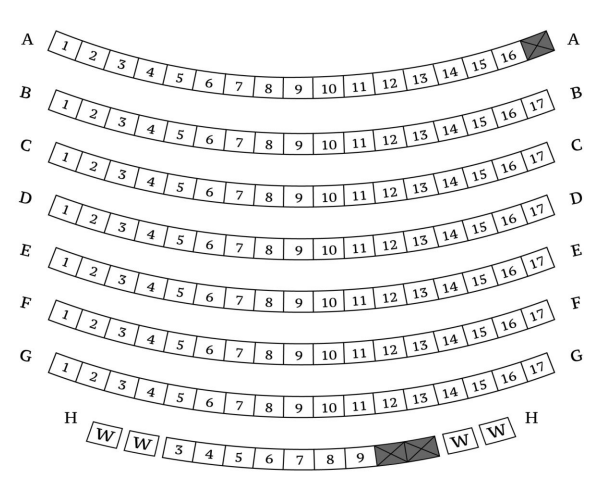
\includegraphics[width=0.6\textwidth]{./Figures/Layouts/Layout_A.png}
    \caption{Layout A}
\end{figure}
  
\begin{figure}[h]
    \centering
      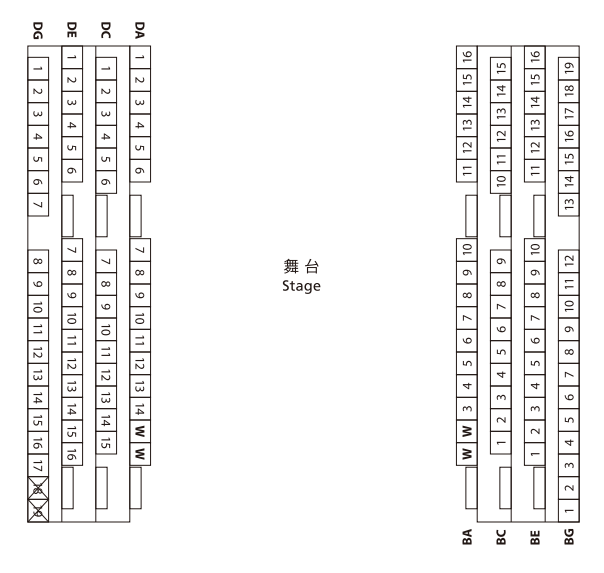
\includegraphics[width=0.6\textwidth]{./Figures/Layouts/Layout_B.png}
    \caption{Layout B}
\end{figure}

\begin{figure}[h]
    \centering
      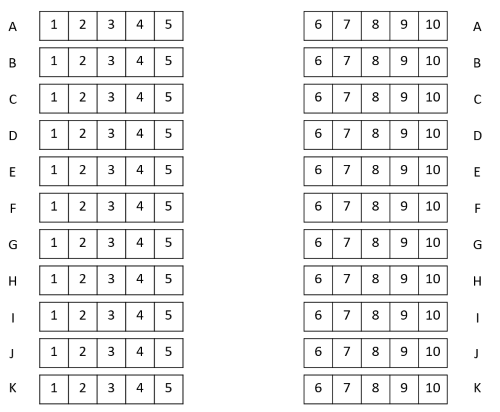
\includegraphics[width=0.6\textwidth]{./Figures/Layouts/Layout_C1.png}
    \caption{Layout C}
\end{figure}

\begin{figure}[h]
    \centering
      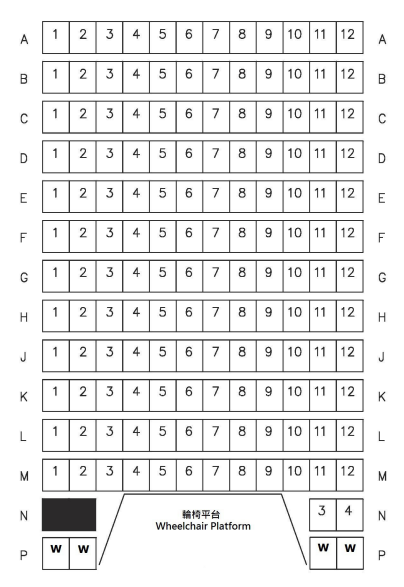
\includegraphics[width=0.6\textwidth]{./Figures/Layouts/Layout_D.png}
    \caption{Layout D}
\end{figure}

\begin{figure}[h]
    \centering
      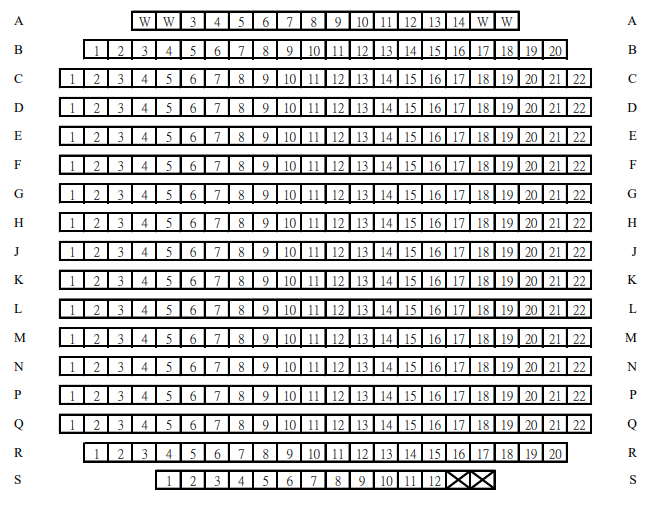
\includegraphics[width=0.6\textwidth]{./Figures/Layouts/Layout_E.png}
    \caption{Layout E}
\end{figure}



% \section{Proof of Theorem 1} \label{sec:ec-proof}
% Here we provide the full proof omitted in the main text...

% \section{Additional Experiments} \label{sec:ec-experiments}
% \subsection{Dataset Details} \label{sec:ec-data}
% The extended dataset is described in Table~\ref{tab:ec-data}.

% % 示例表格
% \begin{table}[ht]
% \centering
% \caption{Extended Dataset Summary} \label{tab:ec-data}
% \begin{tabular}{lc}
% \textbf{Feature} & \textbf{Value} \\
% Size & 10,000 samples \\
% Dimensions & 20 \\
% \end{tabular}
% \end{table}

\printbibliography[title={References in E-Companion}]

\end{document}